\documentclass[13.5pt]{beamer}
\usepackage[natbib=true,backend=bibtex,useprefix=true]{biblatex}
\usepackage[utf8]{inputenc}
\usepackage{tikz}
\usepackage{ragged2e}
\usepackage{adjustbox}
\usepackage{amsmath}
\usepackage{amsfonts}
\usepackage{amssymb}
\usepackage{amsthm}
\usetikzlibrary{fadings}
\usepackage{fontspec}
\usepackage{unicode-math}
\setmathfont{XITS Math}


\usetheme{Madrid}

\definecolor{TorVergataColor}{RGB}{0,125,52}
\setsansfont[BoldFont={Circe-Bold}]{Circe-Regular}

\newcommand{\B}[1]{\textcolor{TorVergataColor}{\textbf{#1}}}
\newcommand{\Cross}{\mathbin{\tikz [x=2.5ex,y=2.5ex,line width=.10ex] \draw (0,0) -- (1,1) (0,1) -- (1,0);}}
\newcommand{\mathDef}{\overset{\textit{def}}{=}}
\newcommand{\N}{\mathbb{N}}
\newcommand{\R}{\mathbb{R}}
\newcommand{\Rplus}{\mathbb{R}^+}

\makeatletter
\setbeamertemplate{title page}{%
	\vbox{}
	\vfill
	{\usebeamercolor[fg]{titlegraphic}\inserttitlegraphic\par}
	\begingroup
	\centering
	\begin{beamercolorbox}[sep=8pt,center]{title}
		\usebeamerfont{title}\inserttitle\par%
		\ifx\insertsubtitle\@empty%
		\else%
		\vskip0.25em%
		{\usebeamerfont{subtitle}\usebeamercolor[fg]{subtitle}\insertsubtitle\par}%
		\fi%     
	\end{beamercolorbox}%
	\vskip1em\par
	\vfill%<- added
	\begin{beamercolorbox}[sep=8pt,left]{author}
		\usebeamerfont{author}\insertauthor
	\end{beamercolorbox}
	\vfill%<- added
	\begin{beamercolorbox}[sep=8pt,center]{institute}
		\usebeamerfont{institute}\insertinstitute
	\end{beamercolorbox}
	\vfill%<- added
	\begin{beamercolorbox}[sep=8pt,center]{date}
		\usebeamerfont{date}\insertdate
	\end{beamercolorbox}%
	\vskip0cm%<- changed
	%    
	\endgroup
	\vfill%<- removed
}
\makeatother



\setbeamercolor{structure}{fg=TorVergataColor}
\setbeamerfont{structure}{family=\bfseries,size=\large}

\title[]
{ 
	\textbf{A QoS-Aware Broker \\ for Multi-Provider Serverless Applications}
}

\author[Andrea Graziani (m. 0273395)]{{\Large \textbf{Andrea Graziani}}\\m. $0273395$\\[10mm]{\small 
		\begin{tabular}{l|l}
			\textbf{Supervisor}: & \textit{Valeria Cardellini } \\ 
			\textbf{Tutor}: & \textit{Gabriele Russo Russo}  \\  
\end{tabular}}}

\titlegraphic{
\includegraphics[width=9.5cm,height=2.4cm]{../Images/UniLogo/LogoMacroarea.png}}

\setbeamertemplate{background}{%
	\begin{tikzpicture}[overlay,remember picture]
		\node[scope fading=west,anchor=north west] at ([shift={(2in,-1in)}]current page.north west) {
\includegraphics[width=9cm,height=9cm]{../Images/UniLogo/TorVergataWatermark.png}};
	\end{tikzpicture}
}

\justifying

\setbeamertemplate{frametitle}{%
	\nointerlineskip%
	\begin{beamercolorbox}[wd=\paperwidth,ht=4.0ex,dp=1ex]{frametitle}
		\hspace*{1ex}\insertframetitle%
	\end{beamercolorbox}%
}

\addtobeamertemplate{frametitle}{}{%
	\begin{tikzpicture}[remember picture,overlay]
		\node[anchor=north east,yshift=2pt] at (current page.north east) {
\includegraphics[height=1cm]{../Images/UniLogo/NegativeTorVergataLogo.png}};
\end{tikzpicture}}

\date{May 23, 2022}

%-------------------------------------------------------
% THE BODY OF THE PRESENTATION
%-------------------------------------------------------




\begin{document}

%-------------------------------------------------------
% THE TITLEPAGE
%-------------------------------------------------------

{% % this is the name of the PDF file for the background
\begin{frame}[plain,noframenumbering] % the plain option removes the header from the title page, noframenumbering removes the numbering of this frame only
  \titlepage % call the title page information from above
\end{frame}}

\setbeamertemplate{background}{}

% -------------- %
% -------------- %
\begin{frame}{Serverless Computing: Overview}

\begin{block}{}
	\centering
	My thesis is focused on ``\B{Serverless Computing}".
\end{block}

\vspace{\baselineskip}
It is a development paradigm according to which:
\vspace{\baselineskip}
\begin{itemize}
	\item Administration tasks (provisioning, monitoring, scaling, etc.) are directly managed by the provider.
	\vspace{\baselineskip}
	
	\item Small-granularity billing pricing model: \B{pay-as-you-go}.
	\vspace{\baselineskip}
	\item Cloud application are abstracted as a group of so-called \\ ``\B{Serverless Functions}".
	
	

	
	
\end{itemize}

\end{frame} 
% -------------- %
% -------------- %
\begin{frame}{Serverless Computing: Overview}
	
	\begin{block}{}
		\centering
		What is a serverless function?
	\end{block}
	\vspace{\baselineskip}
	A computation unit implementing a business functionality.
	
	\begin{itemize}
		\item \B{Stateless}
		\item \B{Event-Driven}
		\item \B{Short-Lived}
	\end{itemize}

	\vspace{\baselineskip}
	
\end{frame} 
% -------------- %
% -------------- %
\begin{frame}{Serverless Computing: Overview}
	
	\begin{block}{}
		\centering
		A serverless function is executed inside a containerized environment: the so-called ``\B{Function Instance}".
	\end{block}

	\vspace{\baselineskip}
	
	\begin{block}{}
		\centering
		The FaaS platform \B{Automatically} scales the number of function instances.
	\end{block}

	\vspace{\baselineskip}
	
	\begin{block}{}
		FaaS platforms impose a \B{Limit} on the number of function instance runnable at the \B{Same Time} called \B{Concurrency Limit}.
	\end{block}

\vspace{\baselineskip}

\begin{block}{}
	A delay is observed when a new function instance is started by the provider: this event is called \B{Cold Start}.
\end{block}
		
\end{frame} 
% -------------- %
% -------------- %
\begin{frame}{Serverless Computing: Overview}
	
	\begin{block}{}
		\centering
		To invoke a \B{serverless function}, users have to specify a so-called \B{serverless function configuration}.
	\end{block}
	\vspace{\baselineskip}
	\begin{block}{}
		\centering
		To invoke a \B{serverless application}, users have to specify a configuration for \B{all} its functions.
	\end{block}
	\vspace{\baselineskip}
	\begin{block}{}
		\centering
		Configuration parameters \B{significantly} affect the \B{cost} and \B{response time} of serverless functions.
	\end{block}
	
	
\end{frame} 
% -------------- %
% -------------- %
\begin{frame}{Serverless Computing: Problems}
	
	\begin{itemize}
		\item The fulfillment of \B{Non-Functional Requirements} concerning the \B{Quality of Service} (QoS) levels that should be guaranteed for 
		any \B{generic} serverless workflow.
		\vspace{\baselineskip}
		\item The lack of support for application whose functions are hosted on \B{Multiple Providers}.
		\vspace{\baselineskip}
		\item The lack of support for serverless function implementations abstraction, that is, for the so-called \B{Concrete Functions}.
		\vspace{\baselineskip}
		\item The fulfillment of \B{Functional Requirements} concerning the \B{orchestration} of \B{Multi-Provider, Multiple-Implementation Serverless Applications}.
	\end{itemize}

\end{frame} 
% -------------- %
% -------------- %
\begin{frame}{State of Art}

Solutions concerning QoS fulfillment \B{already exist}.
\vspace{\baselineskip}
\begin{itemize}
	\item Despite there are some exceptions, they are unaware of both the current status of FaaS platforms and user traffic.
	\vspace{\baselineskip}
	\item Some solutions provide no support for generic workflow.
	\vspace{\baselineskip}
	\item No support for Multi-Provider and Multiple-Implementations serverless applications. 
		\begin{itemize}
			\item No one provides an analytical model to evaluate their performance.
		\end{itemize}
	\vspace{\baselineskip}
	\item Many solutions rely on QoS-aware scheduling algorithms while others rely on the formulation and solving of optimization problems.
\end{itemize}

\end{frame} 

% -------------- %
% -------------- %

\begin{frame}{Thesis Goals}
	
	\begin{block}{Goal $\#$ 1}
		\centering
	To guarantee the \B{Satisfaction of QoS Levels} for Multi-Provider and Multiple-Implementations serverless applications. 
	\end{block}

	\vspace{\baselineskip}
	It was necessary to develop:
	\vspace{\baselineskip} 
	
	\begin{enumerate}
	
		\item An \B{Analytical Model} to evaluate applications performance.
		\begin{itemize}
			\item Supporting generic workflow (branch, loop, parallel)
			\item Providing support for Multi-Provider, Multiple-Implementation Serverless Applications
			\item FaaS-Status-Aware.
		\end{itemize}
		
		
		\vspace{\baselineskip} 
		
	\end{enumerate}
	\end{frame} 

% -------------- %
% -------------- %

\begin{frame}{Thesis Goals}
	
	\begin{enumerate}
		\justifying
		\setcounter{enumi}{1}
		\item A \B{Methodological Way} to find the ``best" configuration to satisfy QoS constraints.
		\begin{itemize}
			\item By solving an \B{Optimization Problem} (LP).
		\end{itemize}
		
		\vspace{\baselineskip}
		
		\item A custom \B{Heuristic Algorithm} to rapidly resolve the aforementioned optimization problem.
		\begin{itemize}
			\item Based on \B{Ant Colony Optimization} algorithm (ACO) family.
		\end{itemize}
		
	\end{enumerate}
	
\end{frame} 

% -------------- %
% -------------- %

\begin{frame}{Thesis Goals}
	
	\begin{block}{Goal $\#$ 2}
		\centering
		The \B{Orchestration} for Multi-Provider and Multiple-Implementations serverless applications. 
	\end{block}
	
	\vspace{\baselineskip}
	To achieve it, I had to build:
	\vspace{\baselineskip}

	\begin{enumerate}
		\justifying
	
		\item A \B{Software Framework}
			\begin{itemize}
				\item Users/Serverless Application Management (CRUD operations, profiling tasks, orchestration task, etc.)
				\item User-Traffic/QoS/FaaS-Status Aware.
			\end{itemize}
		
		\vspace{\baselineskip} 
		\item An extension to an already existent \B{Representation Scheme} to define a serverless application workflow.
		\begin{itemize}
			\item Based on an existing language called \B{Abstract Function Choreography Language} (AFCL).
		\end{itemize}
		
	\end{enumerate}
	
\end{frame} 

% -------------- %
% -------------- %

\begin{frame}{The Prototype}
	
 	Main features of our software framework:
	\vspace{\baselineskip}
	\begin{itemize}
		\item \B{Client-Server architecture}.
		\item \B{Cloud-native} application.
		\item Includes a set of \B{adapters} to interact with following FaaS providers:
		\begin{itemize}
			\item AWS Lambda.
			\item Apache OpenWhisk.
		\end{itemize}
		\item \B{REST} architectural style.
	\end{itemize}
	
\end{frame} 
% -------------- %
% -------------- %
\begin{frame}

\begin{center}
	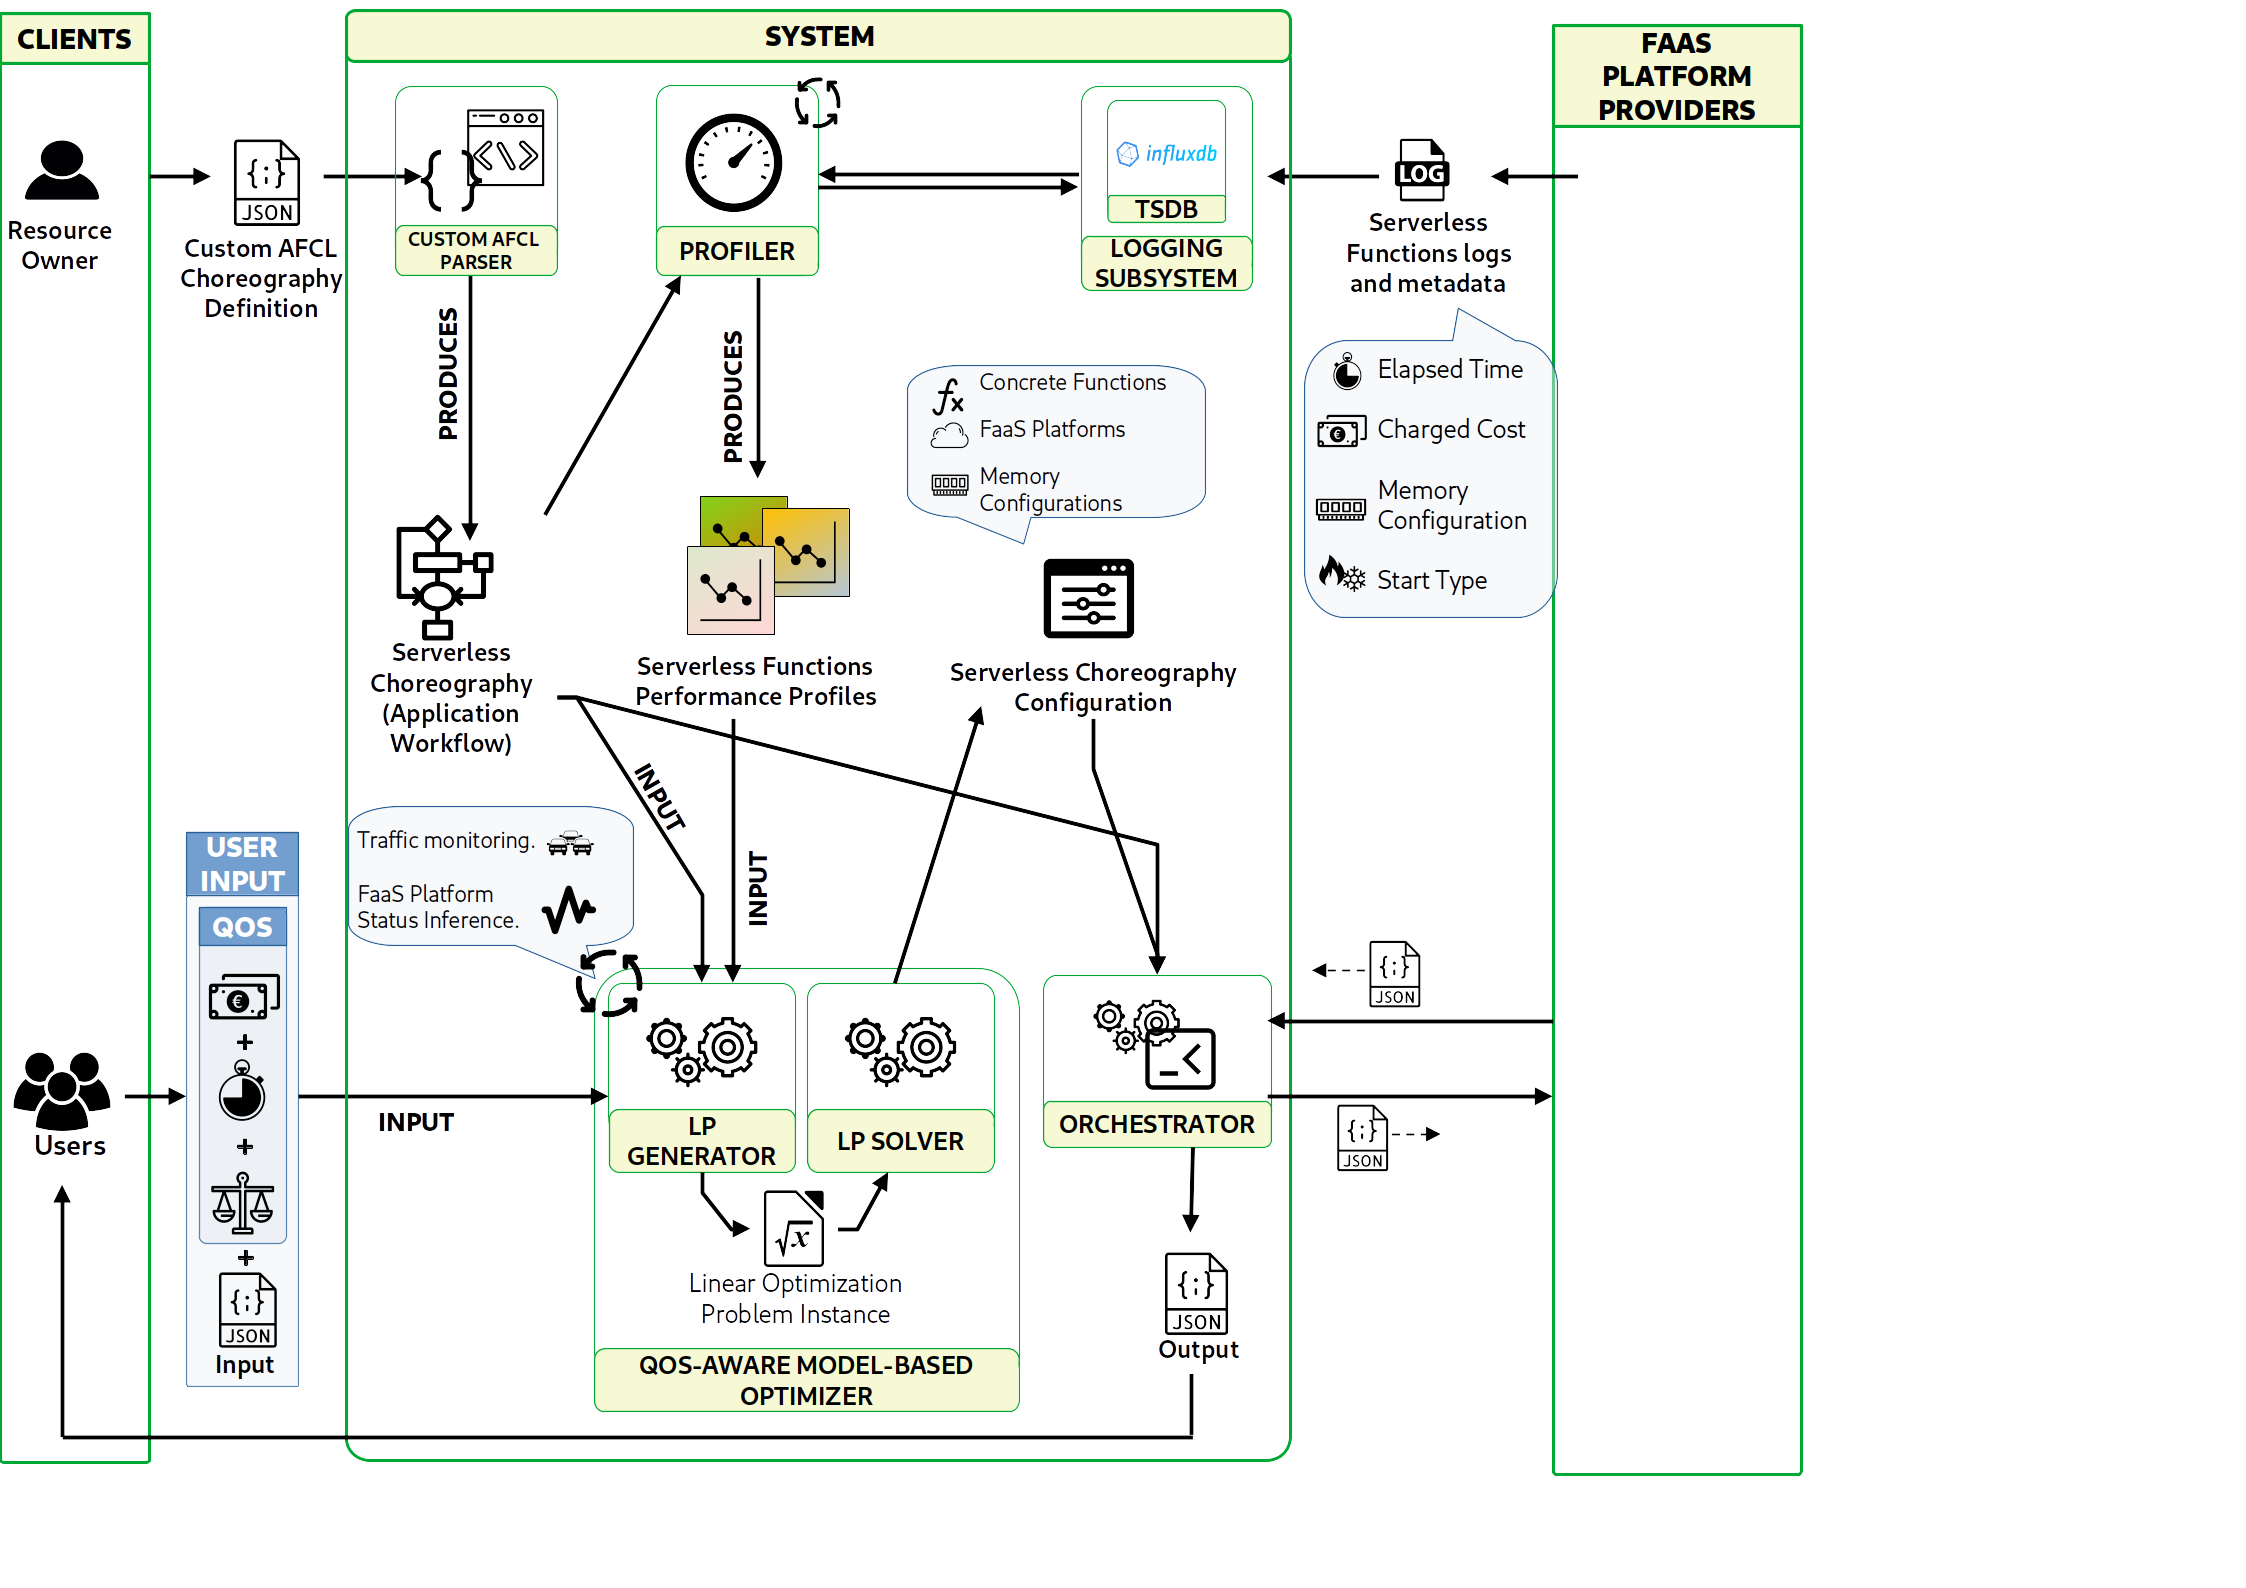
\includegraphics[width=\textwidth,height=0.95\textheight]{../Images/SystemForSlide.png}
\end{center}


\end{frame} 
% -------------- %
% -------------- %
\begin{frame}{The Analytical Model}
	
	\begin{block}{}
		\centering
		Serverless applications are abstracted to a \\\B{Weakly Connected Weighted Directed Graph}.
	\end{block}
	\vspace{\baselineskip}
	\begin{itemize}
		\item Each \B{vertex} models an \B{abstract serverless function}.
		\begin{itemize}
			\item To each abstract function corresponds a set containing all concrete function implementing it.
		\end{itemize}
		\vspace{\baselineskip}
		\item Each \B{edge} represents the calling relationship between two abstract functions. 
		\begin{itemize}
		\item Edge weights represent the so-called \B{transition probability}. 
		 \end{itemize}
		
	\end{itemize}
		
\end{frame} 
% -------------- %
% -------------- %
\begin{frame}{The Analytical Model}
	
	
	\begin{block}{}
		The model provides algorithms and equations to evaluate the performance of a \B{serverless application} under a given configuration.
	\end{block}
	\vspace{\baselineskip}
	
	Aforementioned algorithm depends on:
	\begin{itemize}
		\item The topological properties of the graph representing the application.
		\item The actual value of transition probabilities of all edges.
		\item The estimation of concrete function performance.
	\end{itemize}
	
\end{frame}
% -------------- %
% -------------- %
\begin{frame}{The Analytical Model}

To evaluate the performance of a concrete function is required:
\vspace{\baselineskip}
\begin{itemize}
	\item An estimations about the \B{Average Response Time} (\B{Cost}) in case of cold (warm) start are required.
	\begin{itemize}
		\item To compute aforementioned estimations, \B{Exponential Moving Average} based approach is adopted.
	\end{itemize}
	\vspace{\baselineskip}
	\item An estimation of the probability according to which a request follows a cold start (\B{Cold Start Probability})
\end{itemize}

\end{frame} 
% -------------- %
% -------------- %
\begin{frame}{The Analytical Model}
	
	\begin{block}{}
	Any FaaS platform provider is modeled by set of $M/G/K(t)_{\textbf{C}_{max}}/K(t)_{\textbf{C}_{max}}$ queueing systems.
	\begin{itemize}
		\item $K(t)$: the number of function instances at time $t$.
		\item $C_{max}$: the concurrency limit.
	\end{itemize}
	\end{block}
	
	\begin{block}{}
		\centering
		To compute the cold start probability the \B{Erlang-B} formula is used.
	\end{block}
		
\end{frame}
% -------------- %
% -------------- %
\begin{frame}{}
	
\begin{figure}[h]
	\centering
	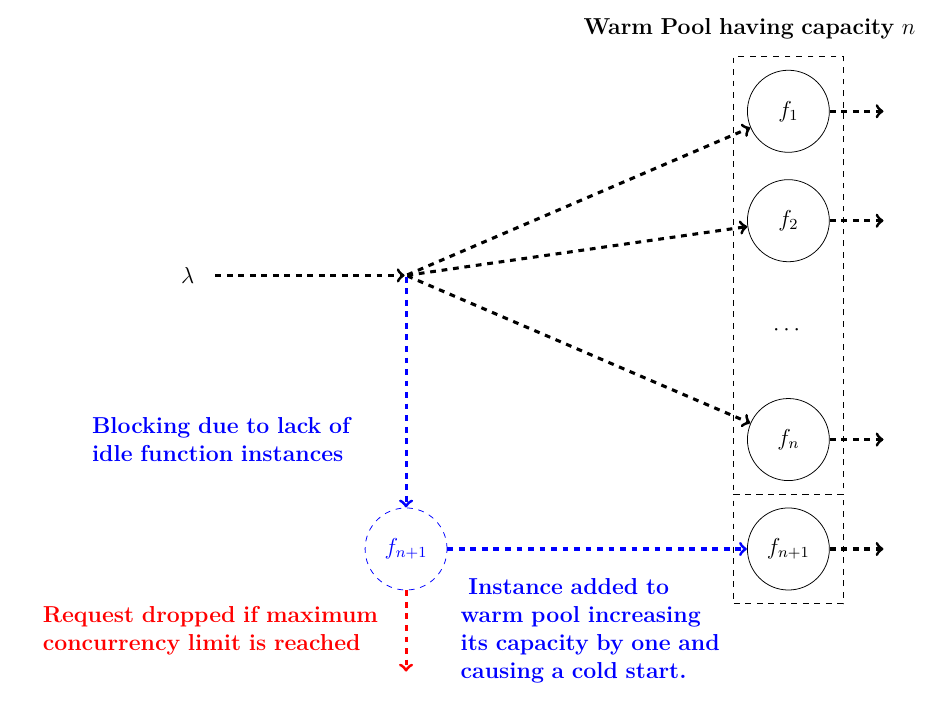
\includegraphics[width=\textwidth]{../Images/FaaSForSlide.png}
\end{figure}
	
\end{frame} 
% -------------- %
% -------------- %

% -------------- %
% -------------- %
\begin{frame}{The Optimization Problem}

\begin{itemize}
	\item To achieve our goal consisting in finding the best configuration to guarantee QoS constraints, we have to solve an \B{optimization problem}.
	\begin{itemize}
		\item It is based on \B{Multi-Dimensional Multi-Choice Knapsack Problem Formulation}. 
	\end{itemize}
\end{itemize}

\end{frame}


\begin{frame}{The Optimization Problem}
	Formally, the configuration vector $\textbf{x}_{\mathcal{C}}$ we want to find is such that:
	
	\begin{eqnarray}
		\textbf{x}_{\mathcal{C}} & \mathDef & \left\lbrace x_{\phi_{1}}, \ldots, x_{\phi_{k}} \right\rbrace \nonumber \\ 
		& \in & \left\{  \left\{ \bigcup_{j=1}^{|\textbf{F}_{\phi_{1}}|} f_{\phi_{1_j}} \times \textbf{M}_{f_{\phi_{1_j}}} \right\} \times \ldots \times \left\{ \bigcup_{j=1}^{|\textbf{F}_{\phi_{k}}|} f_{\phi_{k_j}} \times \textbf{M}_{f_{\phi_{k_j}}} \right\} \right\}  \nonumber \\
		& = & \Cross_{i = 1}^k \left\{ \bigcup_{j=1}^{|\textbf{F}_{\phi_{i}}|} f_{\phi_{i_j}} \times \textbf{M}_{f_{\phi_{i_j}}} \right\} \nonumber \\
		& \subseteq & \Cross_{i = 1}^k \left\{ \textbf{F}_{\phi_{i}} \times \mathbb{N} \right\} = \textbf{X}_{\mathcal{C}}
	\end{eqnarray}

\end{frame}

% -------------- %
% -------------- %

\begin{frame}
	
\begin{figure}[h]
	\centering
	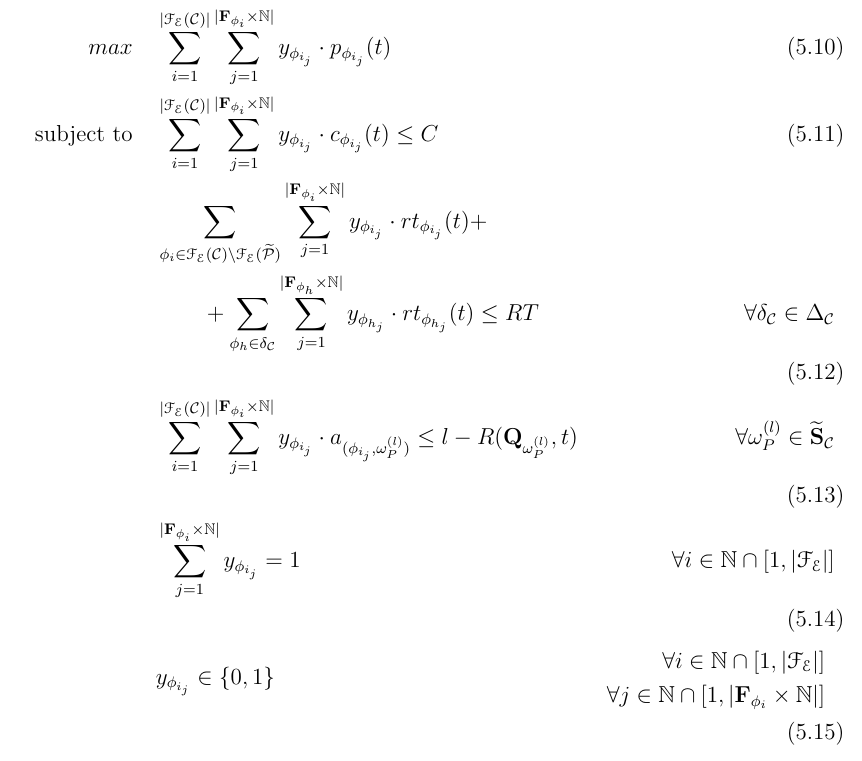
\includegraphics[width=\textwidth,height=0.8\columnwidth]{../Images/MMKPForSlide.png}
\end{figure}
	
	
\end{frame}



% -------------- %
% -------------- %
\begin{frame}{The Heuristic Algorithm}
	
	\begin{block}{}
		\centering
		I develop a custom heuristic algorithm based on \B{Ant Colony Optimization} (ACO); it is called \B{Pre-provisioned Colony Optimization Algorithm with Lazy Pheromone Update}.
	\end{block}
	\vspace{\baselineskip}
	\begin{itemize}
		\item It is based on a set of computational agents, called \B{artificial ants}, which \B{iteratively} construct a solution.
		
		\vspace{\baselineskip}
		
		\item At each iteration, each agent moves from a solution to another, applying a series of stochastic \B{local} decisions whose policy is based on following parameters:
		
		\begin{itemize}
			\item \B{Attractiveness}.
			\item \B{Pheromone Trail}.
		\end{itemize}
		
	\end{itemize}
	
	
	
	
\end{frame}
% -------------- %
% -------------- %
\begin{frame}{The Heuristic Algorithm}
	
	\begin{block}{}
		\centering
		Pheromone trails are updated during \B{every iteration}.
	\end{block}

	\begin{block}{}
		\centering
		Pheromone trails are used to decide which solutions should be preferred during \B{next iterations}.
	\end{block}

	\vspace{\baselineskip}

	\begin{itemize}
		\item A \B{Lazy Approach} for pheromone trails update is used.
		
		\vspace{\baselineskip}
		
		\item A \B{Pre-Provisioning Tactic} is used to anticipates data needs assuring a \B{lower latency}.
	\end{itemize}



\end{frame}
% -------------- %
% -------------- %
\begin{frame}
	
	\begin{figure}[h]
		\centering
		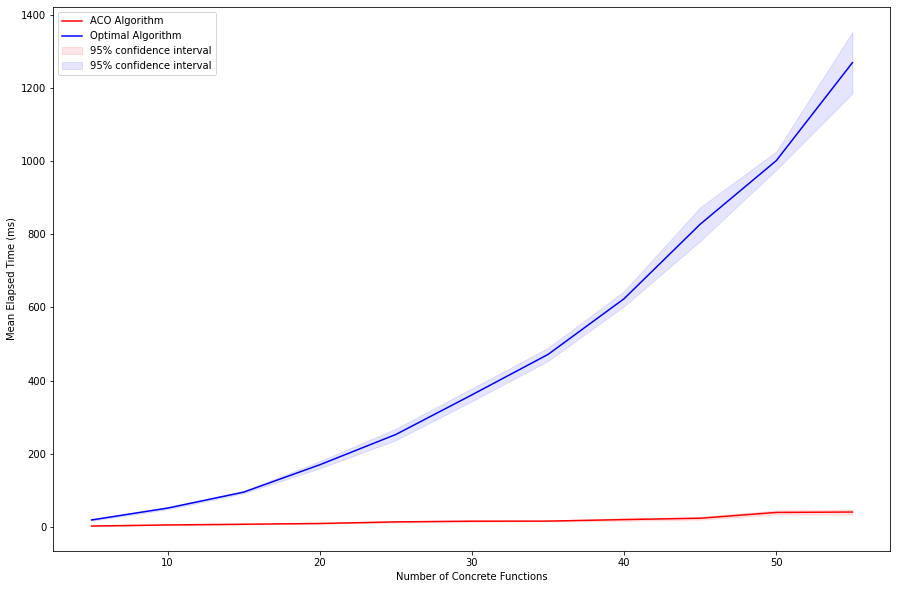
\includegraphics[width=\textwidth, height=0.8\textheight]{../Images/ACOvsOptimalIncreasingConcrete.png}
	\end{figure}
	
\end{frame}

% -------------- %
% -------------- %

\begin{frame}
	
	\begin{figure}[h]
		\centering
		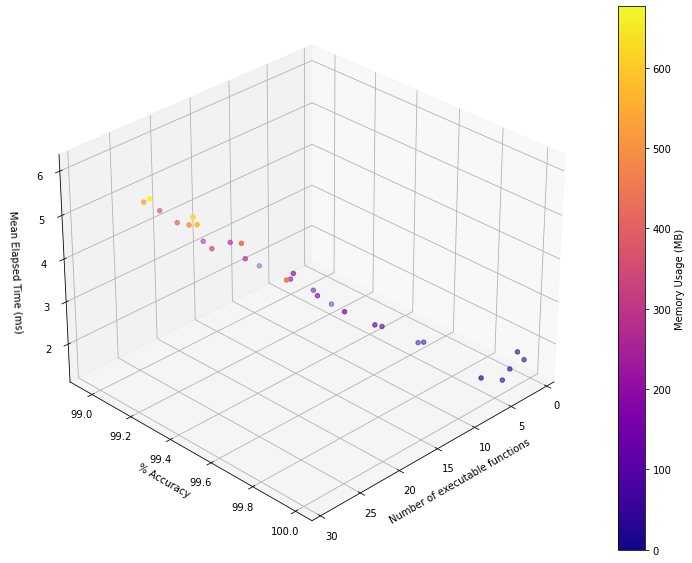
\includegraphics[width=\textwidth, height=0.8\textheight]{../Images/ACO3DIncreasingExecutable.png}
	\end{figure}
	
\end{frame}

\begin{frame}{Conclusions}

\begin{itemize}
	
	\item I presented an analytical model to compute the performance  of a generic serverless workflows having multiple concrete functions hosted on multiple FaaS providers. 
	\vspace{\baselineskip}
	\item I defined an optimization problems formulation to address the problem of finding a suitable configuration in order to meet user defined QoS constraints
	\vspace{\baselineskip}
	\item We developed a heuristic algorithm to rapidly solve it.
	\vspace{\baselineskip}
	\item We verified the validity of both the proposed algorithms and the analytical model through test and experimental evaluations developing a prototype supporting AWS and OpenWhisk.
	
\end{itemize}
\end{frame}

\setbeamertemplate{background}{%
	\begin{tikzpicture}[overlay,remember picture]
		\node[scope fading=west,anchor=north west] at ([shift={(2in,-1in)}]current page.north west) {
\includegraphics[width=9cm,height=9cm]{../Images/UniLogo/TorVergataWatermark.png}};
	\end{tikzpicture}
}

\begin{frame}{{}}
	\begin{block}{}
		\centering
		Thanks for your attention!\\\B{Questions}?
	\end{block}
\end{frame} 

\end{document}
